
\documentclass{article}
\usepackage{ctex}
\usepackage{amsmath}
\usepackage{graphicx}
\usepackage{float}
\usepackage{array}
 
\title{期权定价实验}
\author{}
\date{February 2023}


\begin{document}

\maketitle


\vspace{2ex}

\section{变量代换}

已知 Black-Scholes 方程
$$\frac{\partial u}{\partial t} + \frac{1}{2}\sigma^2S^2\frac{\partial^2 u}{\partial S^2} + rs\frac{\partial u}{\partial S} - ru = 0$$

其中$(S, t) \in [0, S_{max}] × [0, T]$ ,

欧式看涨期权满足条件:
\begin{equation}
    \left\{
            \begin{array}{lr}
            u(0, t) = 0, & \\
            \vspace{1ex}
            u(S_{max}, t) = S_{max} - K, & \\
            \vspace{1ex}
            u(S, T) = max(S - K, 0). &  
            \end{array}
    \right.
    \nonumber
\end{equation}


\vspace{2ex}

我们首先进行变量代换,令$\tau = t-T$,$x = \ln S$,则原方程可以变为:
$$\frac{\partial u}{\partial \tau} + \frac{1}{2}\sigma^2\frac{\partial^2 u}{\partial x^2} + (r-\frac{1}{2}\sigma^2)\frac{\partial u}{\partial x} - r u = 0$$

边界条件变为:$u(x=0, \tau) = 0$,$u(x=x_{\max}, \tau) = e^{x_{\max}}-K$。

终止条件变为:$u(x,\tau=0) = g(x) = \max(e^x-K,0)$。


\section{构建网格}
我们在计算区域 $[0, x] × [-T, 0]$ 上划分标准网格,记空间方向上步长 $h = \Delta x = \frac{S}{(N + 1)}$,时间方向上步长 $\tau = \Delta t = \frac{T}{M}$。在空间方向上我们已知两个边界的值,而时间方向仅有一个边界条件,因此空间方向比时间方向多离散一个网格,保证最终要求解的网格点数为 $M × N$。

此外,我们使用记号$u_{i,j} \approx u(x_i, t_j) = u(i\Delta x, j\Delta t) = u(ih, j\tau)$,作为数值逼近的解。其中 $i = 0,..., N + 1$,$j = 0,..., M$。需要计算的网格点为 $i = 1,..., N$,$j = 1,..., M$。

\begin{figure}[H]
  \centering
  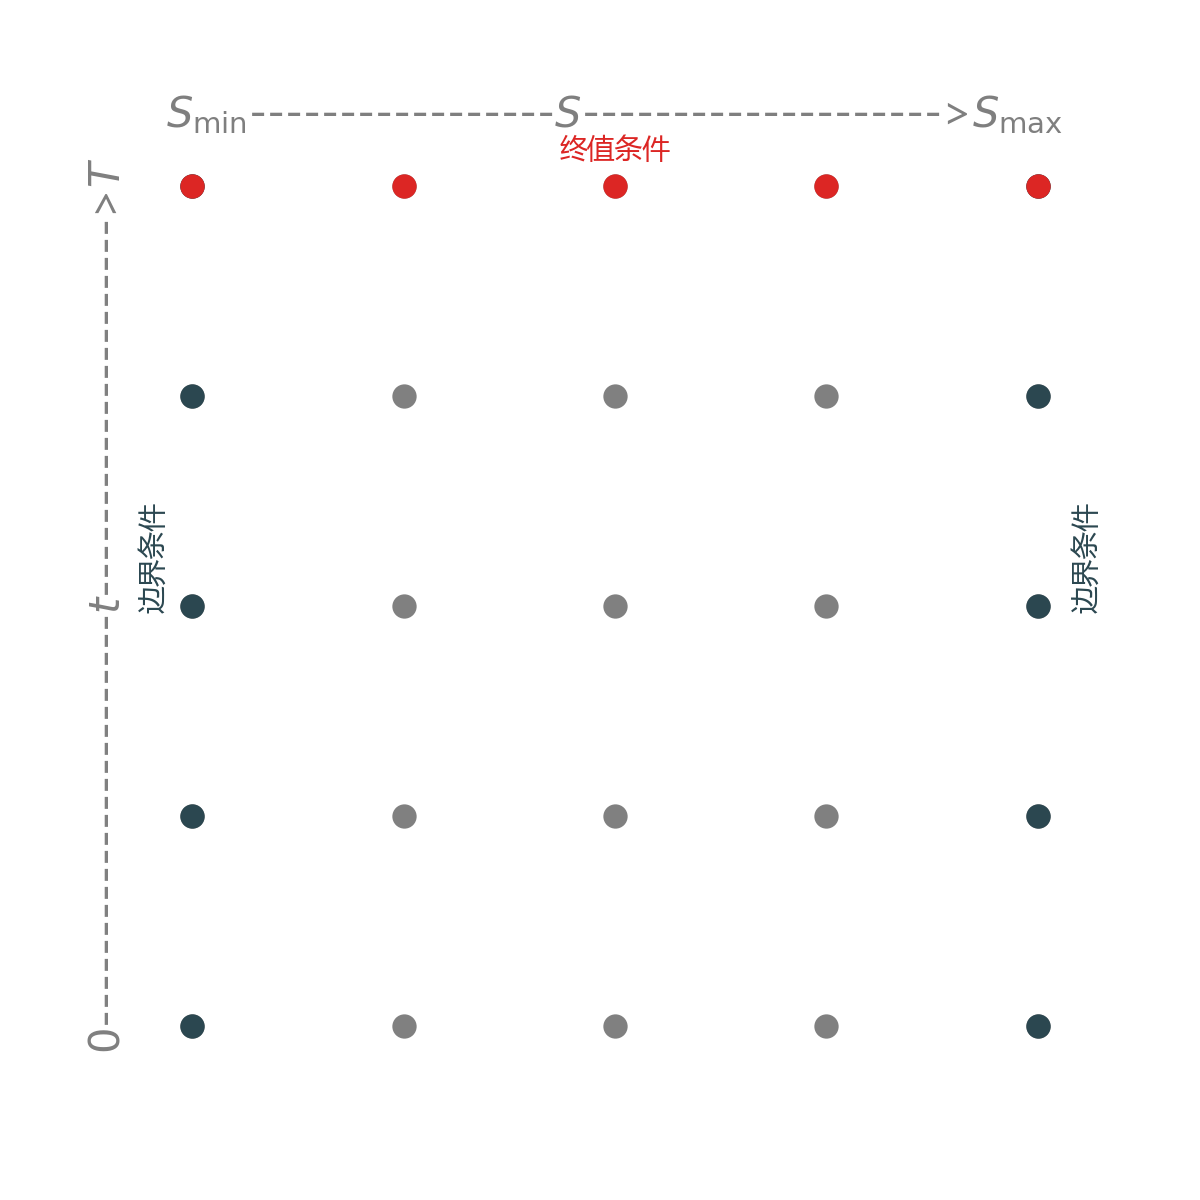
\includegraphics[width=0.64\textwidth,height=0.64\textwidth]{Images/1_grid.png}
  \caption{标准网格}
  \label{fig:1_grid}
\end{figure} 



\section{离散方式}


\subsection{空间方向上的离散}

空间方向采用二阶精度的中心差分
$$\frac{\partial u}{\partial x}(x_i, t_j) = \frac{u_{i+1, j} - u_{i-1, j}}{2h}$$
和
$$\frac{\partial^2 u}{\partial x^2}(x_i, t_j) = \frac{u_{i+1, j} - 2u_{i, j} + u_{i-1, j}}{h^2}$$
作为 Black-Scholes 偏微分方程在空间方向上导数的近似。这样就得到半离散方程
$$\frac{\partial u}{\partial \tau} + (\frac{1}{2}\sigma^2)\frac{u_{i+1, j} - 2u_{i, j} + u_{i-1, j}}{h^2} + (r - \frac{1}{2}\sigma^2)\frac{u_{i+1, j} - u_{i-1, j}}{2h} - ru_{i, j} = 0$$
即$$\frac{\partial u}{\partial \tau} + (\frac{h+2}{4h^2}\sigma^2 - \frac{r}{2h})u_{i-1, j} - (r + \frac{\sigma^2}{h^2})u_{i, j} + (\frac{2-h}{4h^2}\sigma^2 + \frac{r}{2h})u_{i+1, j} = 0$$
为了表示方便,我们令
\begin{equation}
\left\{
        \begin{array}{lr}
        \vspace{1ex}
        a = \frac{h+2}{4h^2}\sigma^2 - \frac{r}{2h}, & \\
        \vspace{1ex}
        b = -(r + \frac{\sigma^2}{h^2}), & \\
        \vspace{1ex}
        c = \frac{2-h}{4h^2}\sigma^2 + \frac{r}{2h}. &  
        \end{array}
\right.
\nonumber
\end{equation}

记$\bar{u}_j = (u_{1, j}, u_{2, j},...,u_{N, j})^T$,当指标$i$取遍$1,2,...,N$时,得到半离散方程组
$$\frac{\partial u}{\partial \tau} + B\bar{u}_j + z = 0, $$
其中$$
B = \begin{pmatrix}
        b &   c    &        &        &   & \\
        a &   b    &   c    &        &   & \\
          & \ddots & \ddots & \ddots &   & \\
          &        & \ddots & \ddots & c & \\
          &        &        &   a    & b & \\
    \end{pmatrix},
\bar{u}_j = \begin{pmatrix}
        u_{1, j}   \\
        u_{2, j}   \\
        \vdots     \\
        u_{N-1, j} \\
        u_{N, j}   \\
    \end{pmatrix},
z = \begin{pmatrix}
        au_{0, j}   \\
        0           \\
        \vdots      \\
        0           \\
        cu_{N+1, j} \\
    \end{pmatrix},
$$





\subsection{时间方向上的离散}

下面我们讨论半离散方程在时间方向上的离散。

我们考虑显式欧拉格式,隐式欧拉格式 和 Crank-Nicolson 格式。





\subsubsection{显式欧拉格式}

在时间方向上的显式欧拉格式为$$\frac{\partial u}{\partial \tau}(x_i, t_j) = \frac{u_{i, j} - u_{i, j-1}}{\tau}$$
代入半离散方程得到:$$\frac{u_{i, j} - u_{i, j-1}}{\tau} + au_{i-1, j} + bu_{i, j} + cu_{i+1, j} = 0$$
$$\Rightarrow u_{i, j-1} = \tau au_{i-1, j} + (1 + \tau b)u_{i, j} + \tau cu_{i+1, j}$$

当指标$i$取遍 $1,...,N$ 时,得到线性方程组$$\bar{u}_{j-1} = (I + \tau B)\bar{u}_{j} + z\tau,$$
其中$\bar{u}_{j} = (u_{1, j}, u_{2, j},...,u_{N, j})^T,$
$$
I + \tau B = \begin{pmatrix}
                1 +\tau b  &   \tau c     &            &            &            & \\
                \tau a     &   1 +\tau b  &   \tau c   &            &            & \\
                           &   \ddots     &   \ddots   &   \ddots   &            & \\
                           &              &   \ddots   &   \ddots   &  \tau c    & \\
                           &              &            &   \tau a   &  1 +\tau b & \\
            \end{pmatrix},
z\tau = \begin{pmatrix}
            \tau au_{0, j}   \\
            0                \\
            \vdots           \\
            0                \\
            \tau cu_{N+1, j} \\
        \end{pmatrix},
$$

\begin{figure}[H]
  \centering
  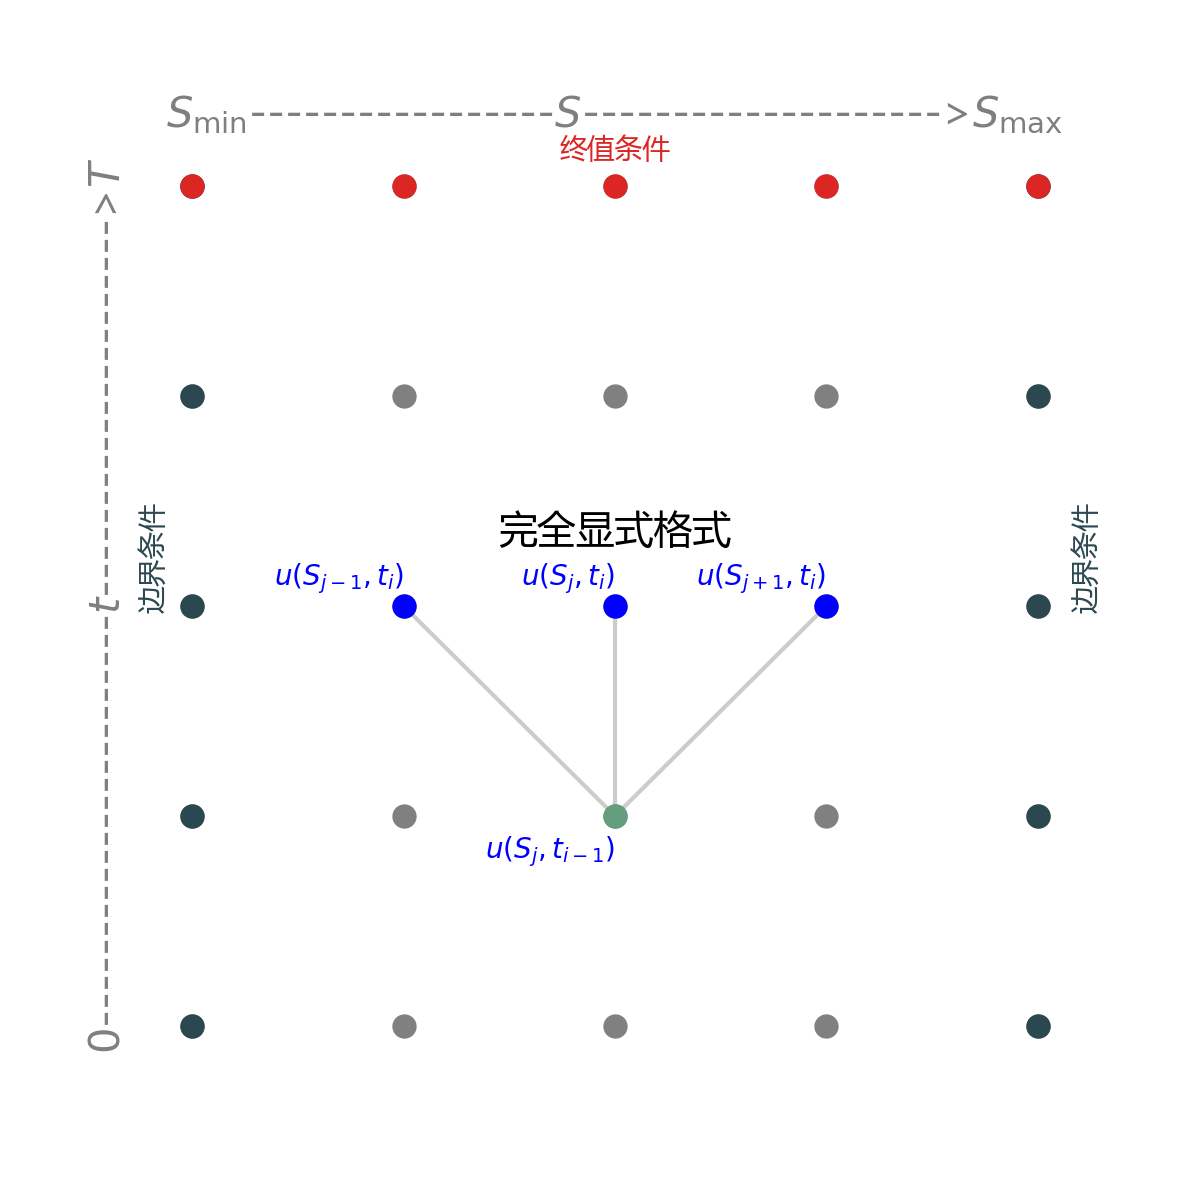
\includegraphics[width=0.64\textwidth,height=0.64\textwidth]{Images/2_ExpEu.png}
  \caption{显式欧拉格式}
  \label{fig:2_ExpEu}
\end{figure} 


\subsubsection{隐式欧拉格式}

在时间方向上的隐式欧拉格式为$$\frac{\partial u}{\partial \tau}(x_i, t_j) = \frac{u_{i, j+1} - u_{i, j}}{\tau}$$
代入半离散方程得到:$$\frac{u_{i, j+1} - u_{i, j}}{\tau} + au_{i-1, j} + bu_{i, j} + cu_{i+1, j} = 0$$
$$\Rightarrow -\tau au_{i-1, j} + (1 - \tau b)u_{i, j} - \tau cu_{i+1, j} = u_{i, j+1}$$

当指标$i$取遍 $1,...,N$ 时,得到线性方程组$$(I - \tau B)\bar{u}_{j} = \bar{u}_{j+1} + z\tau,$$
其中$\bar{u}_{j} = (u_{1, j}, u_{2, j},...,u_{N, j})^T,$
$$
I - \tau B = \begin{pmatrix}
                1 -\tau b  &   -\tau c    &            &            &            & \\
                -\tau a    &   1 -\tau b  &   -\tau c  &            &            & \\
                           &   \ddots     &   \ddots   &   \ddots   &            & \\
                           &              &   \ddots   &   \ddots   &  -\tau c   & \\
                           &              &            &   -\tau a  &  1 -\tau b & \\
            \end{pmatrix},
z\tau = \begin{pmatrix}
            \tau au_{0, j}   \\
            0                \\
            \vdots           \\
            0                \\
            \tau cu_{N+1, j} \\
        \end{pmatrix},
$$


\begin{figure}[H]
  \centering
  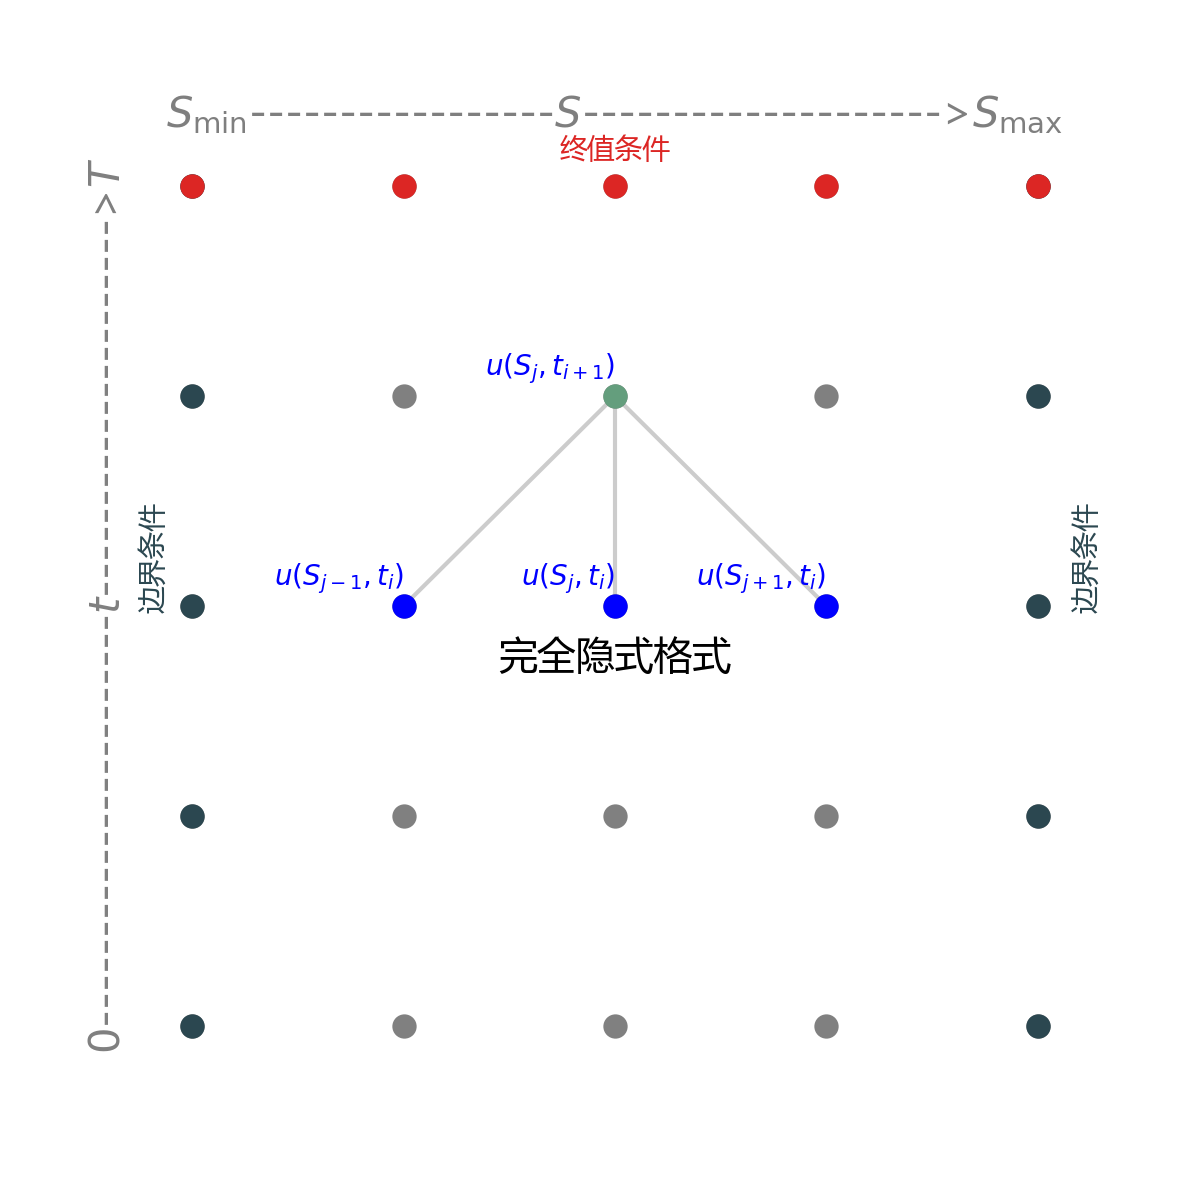
\includegraphics[width=0.64\textwidth,height=0.64\textwidth]{Images/3_ImpEu.png}
  \caption{隐式欧拉格式}
  \label{fig:3_ImpEu}
\end{figure} 






\subsubsection{Crank-Nicolson 格式}

在时间方向上采用中心差分格式,可以看作隐式和显式格式的平均。

将显式欧拉格式的半离散方程中下标$j-1$改成$j$,$j$改成$j+1$,之后将新得到的方程同隐式欧拉格式的半离散方程相加,得到
$$\frac{u_{i, j+1} - u_{i, j}}{\tau} + \frac{1}{2}[(au_{i-1, j} + bu_{i, j} + cu_{i+1, j}) + (au_{i-1, j+1} + bu_{i, j+1} + cu_{i+1, j+1})] = 0$$

同时得到线性方程组$$(2I - \tau B)\bar{u}_{j} = (2I + \tau B)\bar{u}_{j+1} + 2z\tau$$
其中
$$
2I + \tau B = \begin{pmatrix}
                2 +\tau b  &   \tau c     &            &            &            & \\
                \tau a     &   2 +\tau b  &   \tau c   &            &            & \\
                           &   \ddots     &   \ddots   &   \ddots   &            & \\
                           &              &   \ddots   &   \ddots   &  \tau c    & \\
                           &              &            &   \tau a   &  2 +\tau b & \\
            \end{pmatrix},
$$
$$
2I - \tau B = \begin{pmatrix}
                2 -\tau b  &   -\tau c    &            &            &            & \\
                -\tau a    &   2 -\tau b  &   -\tau c  &            &            & \\
                           &   \ddots     &   \ddots   &   \ddots   &            & \\
                           &              &   \ddots   &   \ddots   &  -\tau c   & \\
                           &              &            &   -\tau a  &  2 -\tau b & \\
            \end{pmatrix}.
$$


\begin{figure}[H]
  \centering
  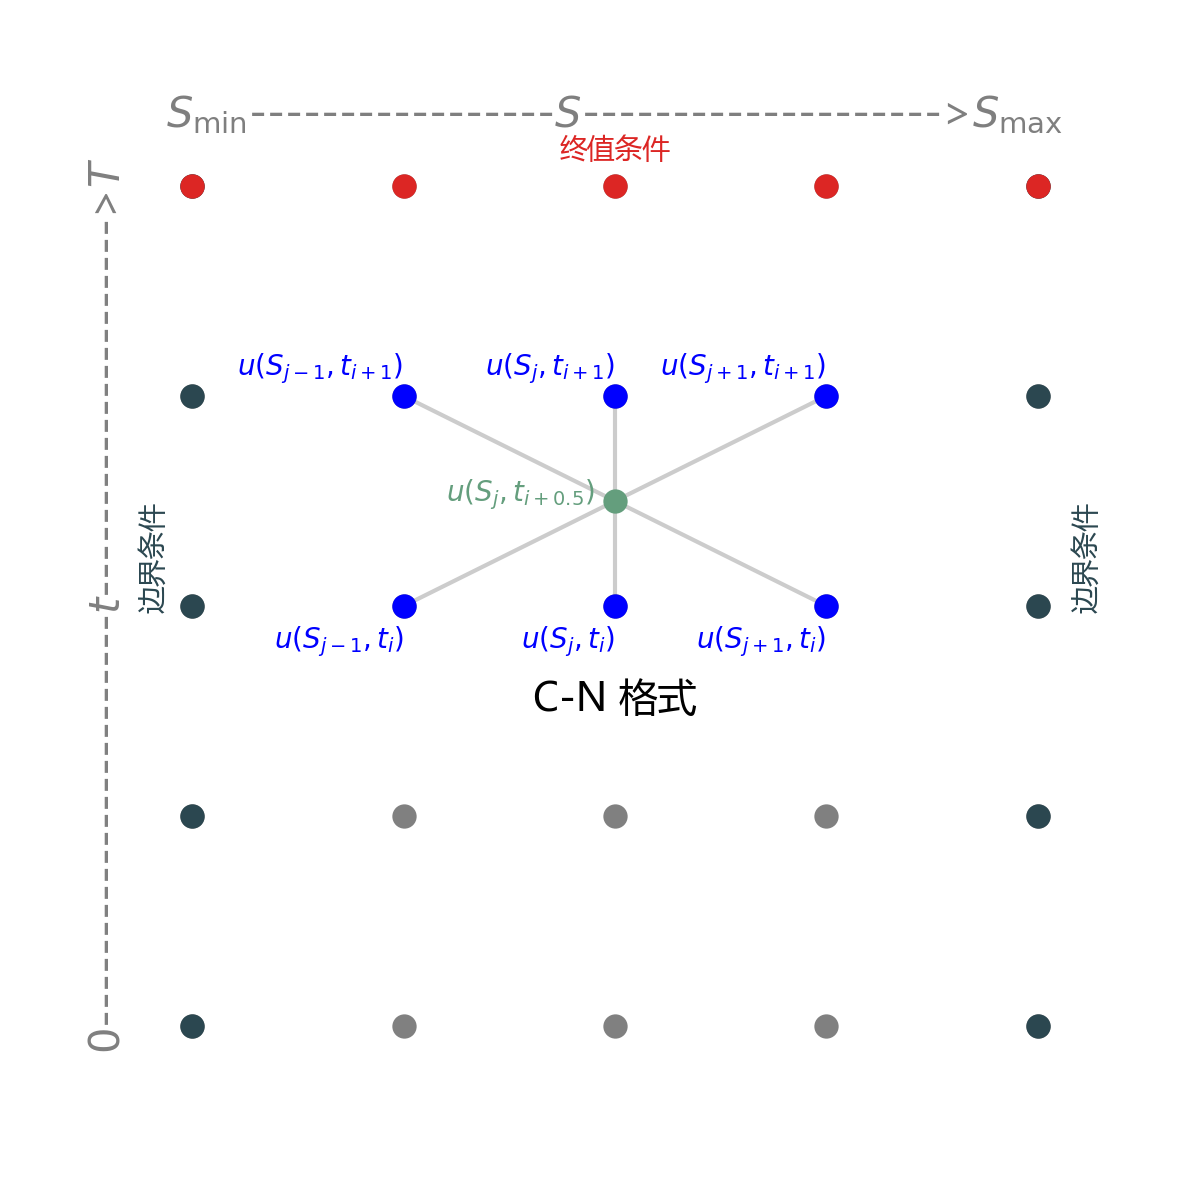
\includegraphics[width=0.64\textwidth,height=0.64\textwidth]{Images/4_CNEu.png}
  \caption{Crank-Nicolson 格式}
  \label{fig:4_CNEu}
\end{figure} 


\section{求解过程可视化}


\begin{table}[h!]
\centering
\begin{tabular}{|c|c|}
\hline
1 & 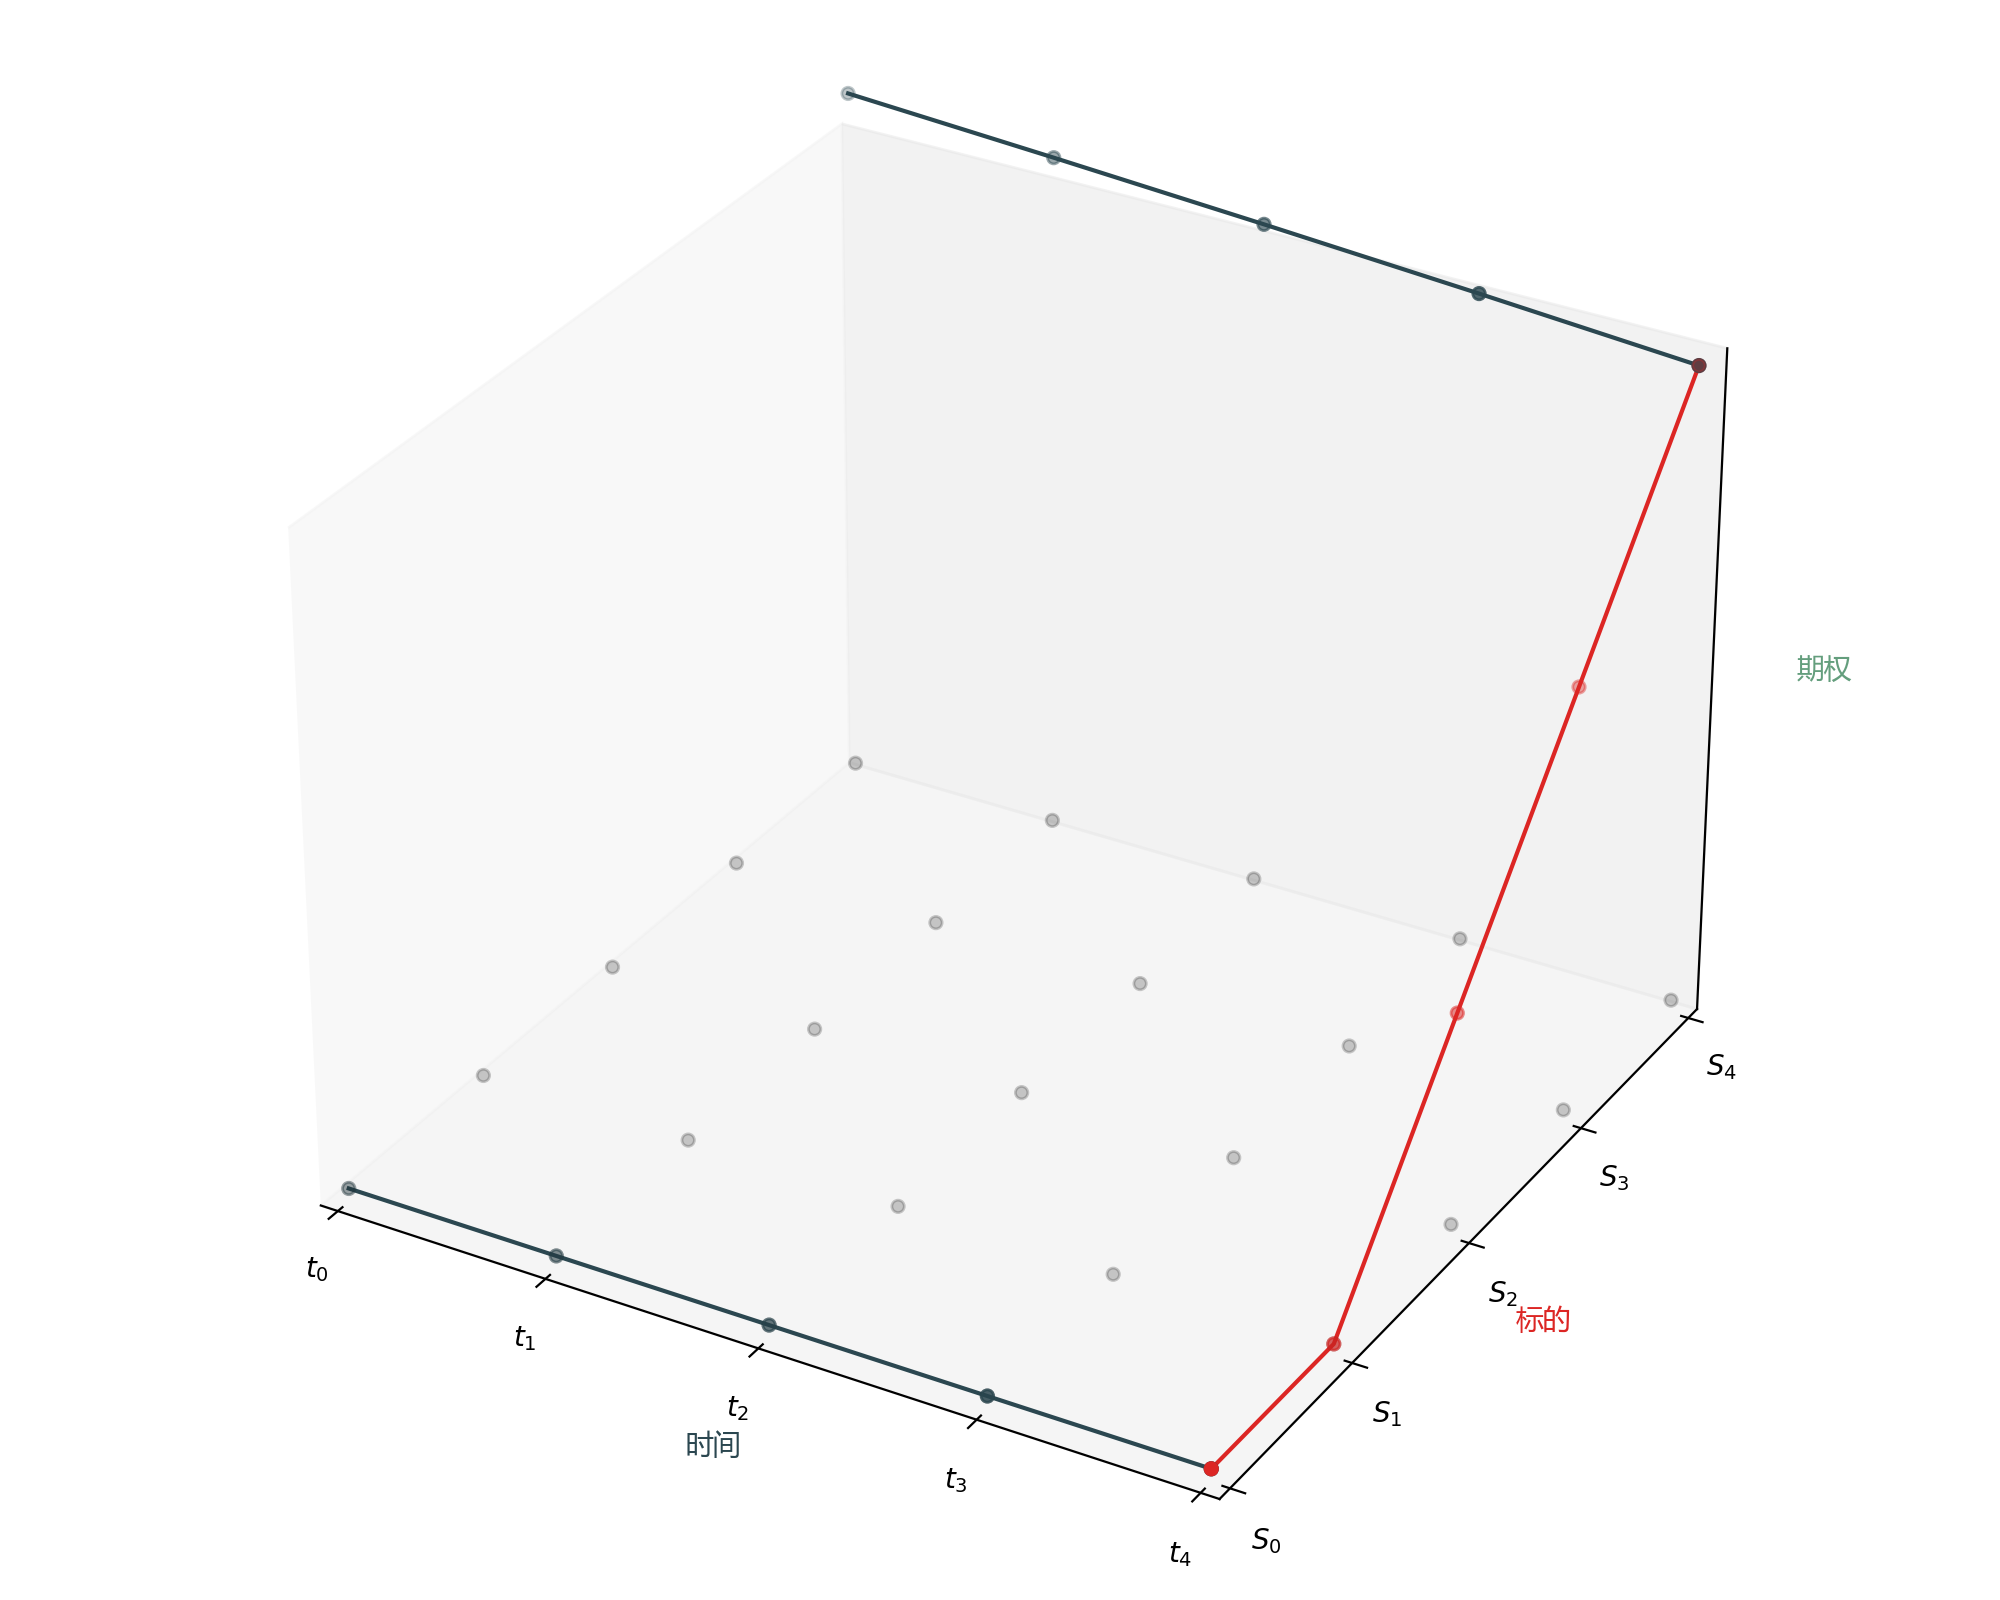
\includegraphics[width=0.4\textwidth]{Images/5_option_price_surface_4iter_step0.png} \\
\hline
2 & 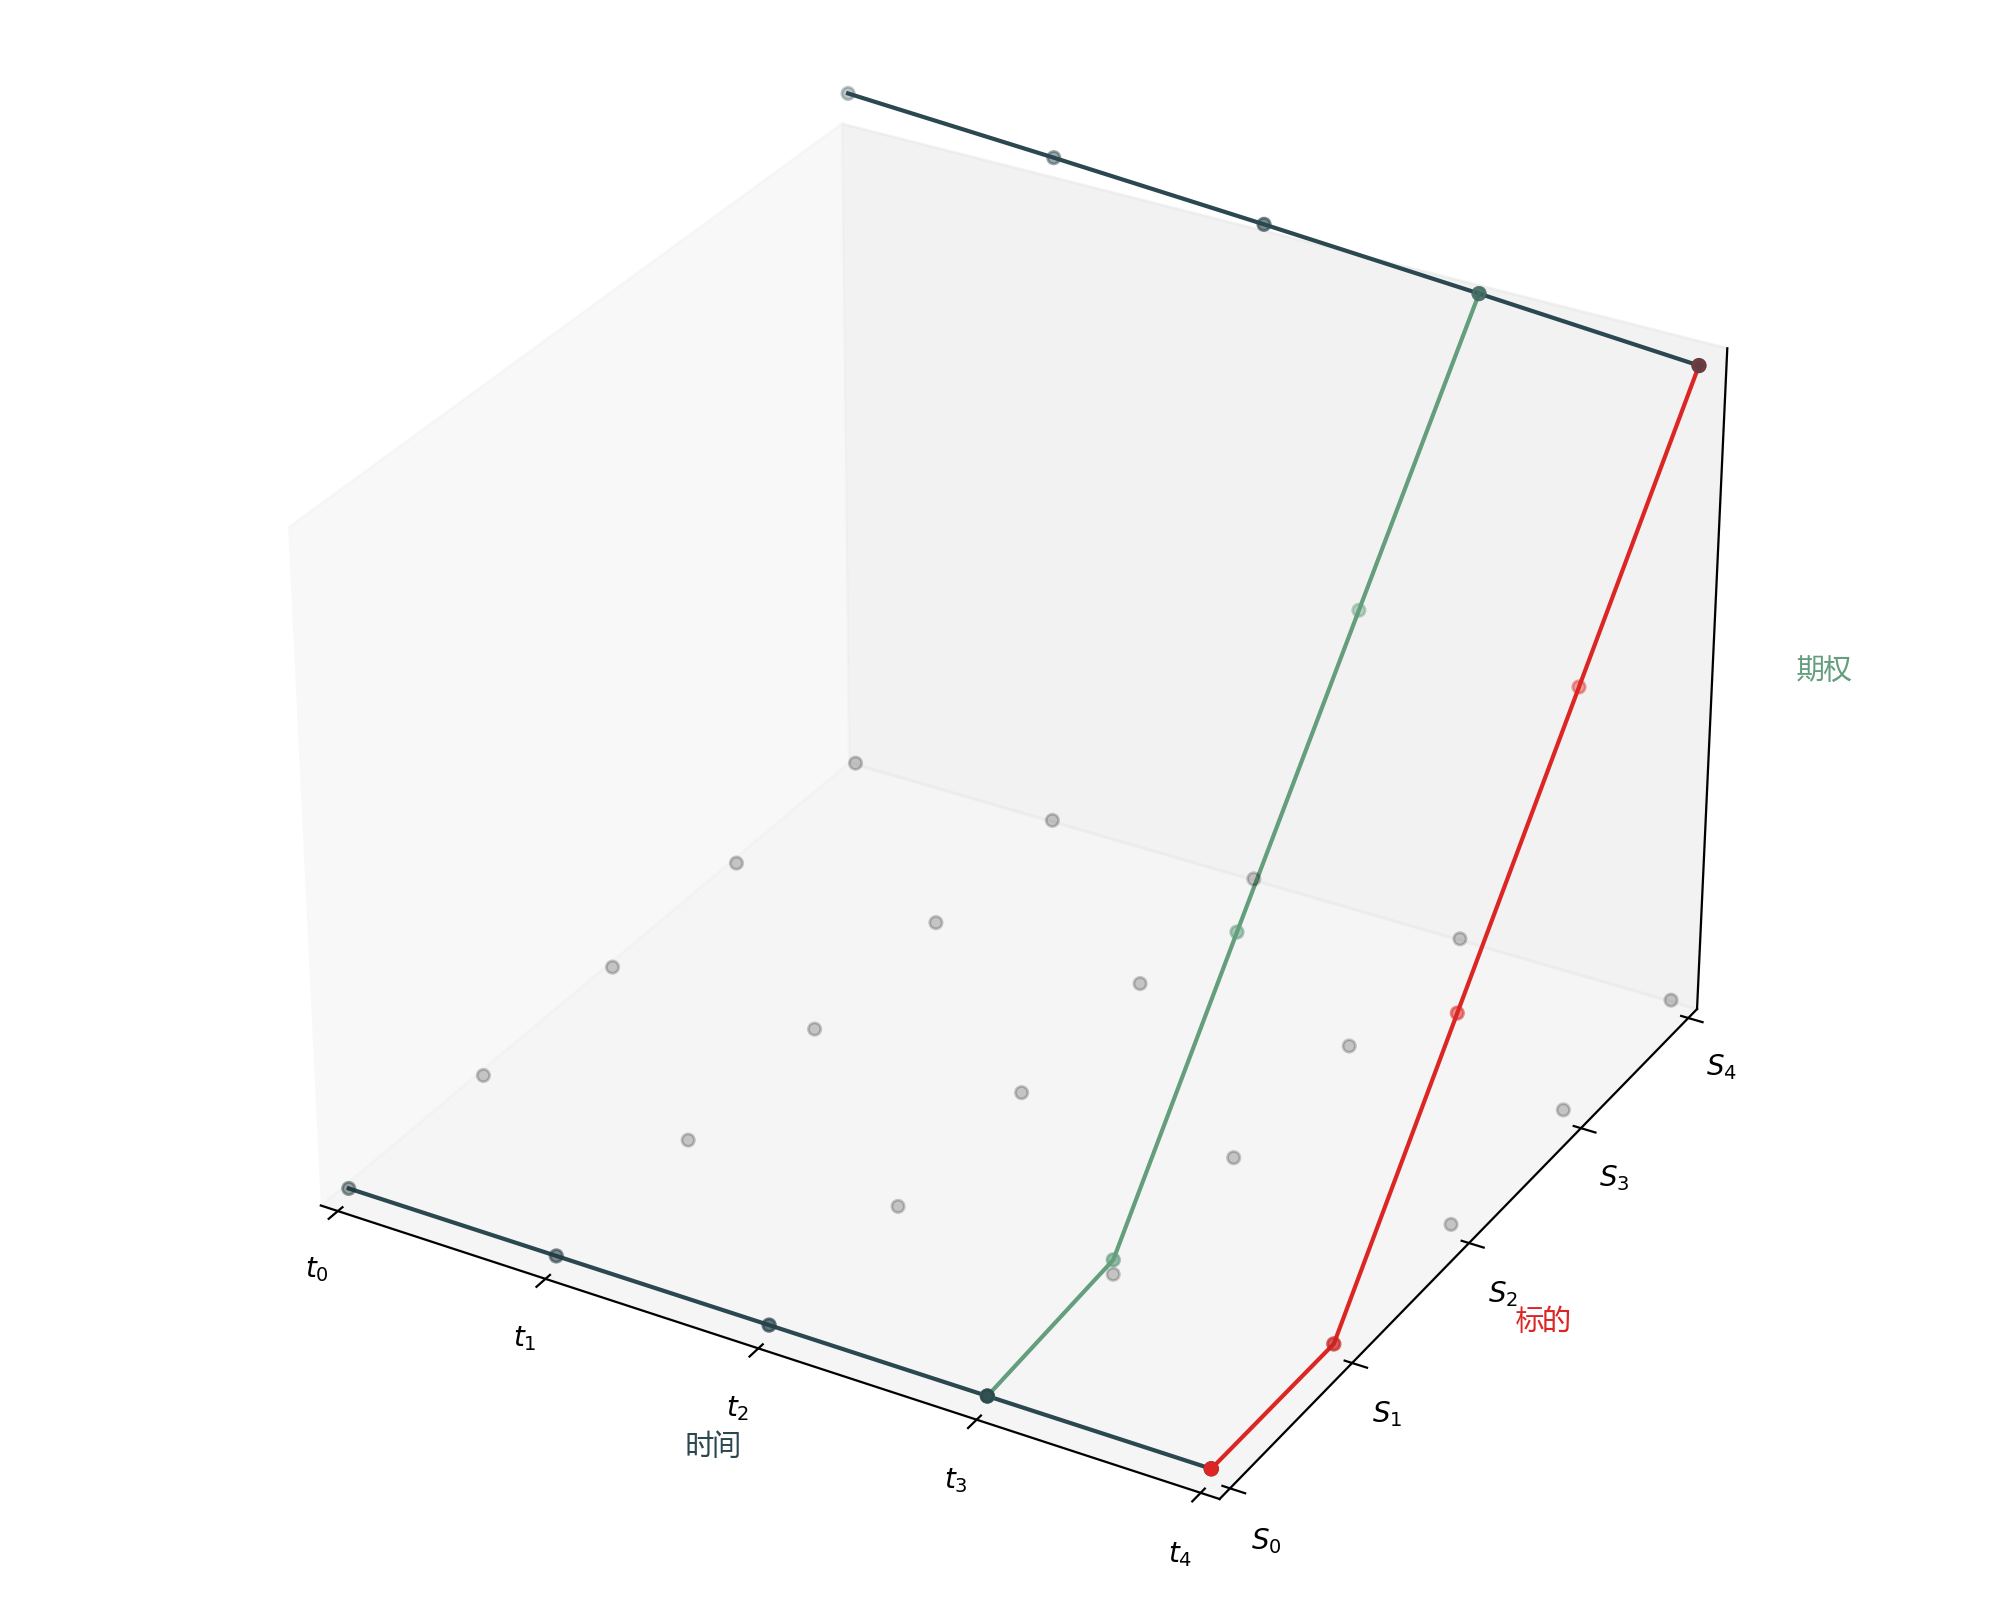
\includegraphics[width=0.4\textwidth]{Images/6_option_price_surface_4iter_step1.png} \\
\hline
\end{tabular}
\caption{一个带有图像的表格示例}
\label{table:example}
\end{table}





\end{document}
